%%%%%%%%%%%%%%%%%%%%%%%%%%%%%%%%%%%%%%%%%%%%%%
\section{Beamline instrumentation}
\label{sec:beaminstruments}

The H4 beamline will be instrumented with a number of beamline monitors to provide information 
 about the beam profile, position, momentum, particle identification, and trigger capability. 
This section discusses the baseline design for the beam monitors. 
\fixme{Is `baseline design' the right term to use?}

%%%%%%%%%%%%%%%%%%%%%%%
\subsection{Beam profile monitoring, particle tracking and momentum measurements}

Operation of the beamline requires at least one beam  monitor, able to provide the beam profile in two dimensions at the end of the beamline.   The beam monitor can also be exploited for data analysis, provided that it delivers data on an event-by-event basis. Another monitor, located immediately downstream of the last bending magnet, is added in the layout  in order to determine the particle  direction and position, and match it with the reconstructed track in the LAr active volume.

The uncertainty in momentum resolution of the beam can be reduced by measuring the momentum particle by particle, with a set of three detectors placed one before and two after one of the bending magnets. In ideal conditions, momentum resolutions of the order of 1\% could be achieved with this system; however since multiple scattering can affect the measurement
at low energies, only a full simulation of the beamline can assess the performance of the setup.  
Preliminary results using full simulations indicate that a momentum resolution on the order of  2\% is achievable. The %same 
devices that are used for beam monitoring can also be used for momentum measurements.
%
\paragraph{Fiber tracker}
The CERN Beam Instrumentation (BI) group will produce
 beam monitors based on scintillating fibers, which have a polystyrene core surrounded by cladding\cite{Scifi}. Fibers provide a light yield of $\sim$8000 photons/MeV, deposited with fast rise and decay times of 1--3 ns. The baseline design foresees 1-mm square fibers in two planes to provide $x$ and $y$ coordinates. Fibers will be mirrored on one end to increase
light collection.  Every monitor consisting of two planes of 1-mm thick fibers adds 0.47\% $X_0$ to the material budget. 
\fixme{$X_0$ mentioned in sec 4.9.7 but not defined anywhere} The tree devices needed for momentum measurement will consist of one layer only, oriented perpendicularly to the magnet deflection.
A fiber plane is made out of 192 fibers with no space between them. It will cover an area of 192~mm $\times$ 192~mm and fits in the beamline.
Scintillation light will be read out by SiPMs, which in turn will be read out by custom electronics depending on the application (see below about the use for Time of Flight).
%
\fixme{Need to decide on one and describe that one. (Anne : meaning some custom elec, which one gets used depends on what sort of application -- what you'll use it for or some s/w app?) }
These monitors are designed to work inside the vacuum chamber and can be mounted on special flanges, without need to break the vacuum.

\paragraph{Multi-wire proportional chambers}
As a backup solution,
Fermilab has multi-wire proportional chambers (MWPCs) with $x-y$ sense plane
readout, measuring approximately 128~mm $\times$ 128~mm, readily available that can also be used as beam profile monitors.  
Chambers add 2\% nuclear collision lengths and 7\% radiation lengths.
 These chambers have a long history, so installation, integration and commissioning should be straightforward. They are operated in air, thus would require dividing the beamline vacuum into sections.


%%%%%%%%%%%%%%%%%%%%%%%
\subsection{Particle identification}

The H4 beamline is capable of delivering two types of beams, electron and hadron. % beams. 
While the electron beam is relatively pure, the hadron beam consists of a mixture of electron, pion, kaon, and proton. Therefore it is essential to have an efficient particle identification system to cleanly tag particle types on a particle-by-particle basis. To achieve this goal, a particle identification system based on a combination of threshold Cherenkov counters and time-of-flight (ToF) system is envisaged for ProtoDUNE-SP. 
\fixme{Again, "is being considered" is not appropriate for a TDR (Anne: is `envisaged' any better? Is it actually planned at this point?)}
Cherenkov counters can be placed in the last segment of the beamline, between the last bending magnet and the cryostat. Space for a ToF system is available, provided that the detector envelope along the beamline is limited to 10 -- 20~cm,
and would allow a flight path of 23~m.
\fixme{Will readers know what the ``detector envelope along the beamline'' is? I don't (Anne)}

\paragraph{Threshold Cherenkov counter}
The threshold Cherenkov counters have been used extensively in beamlines to discriminate particles. Figure~\ref{fig:ckv} shows one of the counters used in the CERN test beam area. It consists of a gas radiator that is contained in a long cylindrical tube, and a detection box in which the Cherenkov light is reflected by a 45$^\circ$ mirror and focused onto a photomultiplier tube. The diameter of the cylindrical tube is designed to allow the counter to pass through the standard CERN beam pipe of about 20cm. A variety of gasses (e.g. CO2, nitrogen, argon, Freon 12, air) are available at CERN to optimize particle identification. 
Two threshold Cherenkov counters will be installed in the beamline, one detecting pions, the other detecting pions 
and kaons. The combination of the two signals will allow to identify all hadron species. In order to provide signals at low beam momenta, either high density gases or high pressures are needed.
%The CERN beam group plans to install at least one (possibly two) threshold Cherenkov counter in the H4 beamline. 
%\fixme{Cannot be written as is; need to describe benefit of one vs two threshold Cherenkov counters; baseline is presumably one counter; so, describe one and then say that there mat=y be additional benefits (which ?) if a second one is added.}
Figure~\ref{fig:ckv_gases} shows the gas pressure threshold 
for the production of Cherenkov light for various particle types as a function of particle momentum for Freon 12 and CO$_2$ gases.
\begin{cdrfigure}[CERN threshold Cherenkov counter]{ckv}{CERN threshold Cherenkov counter}
  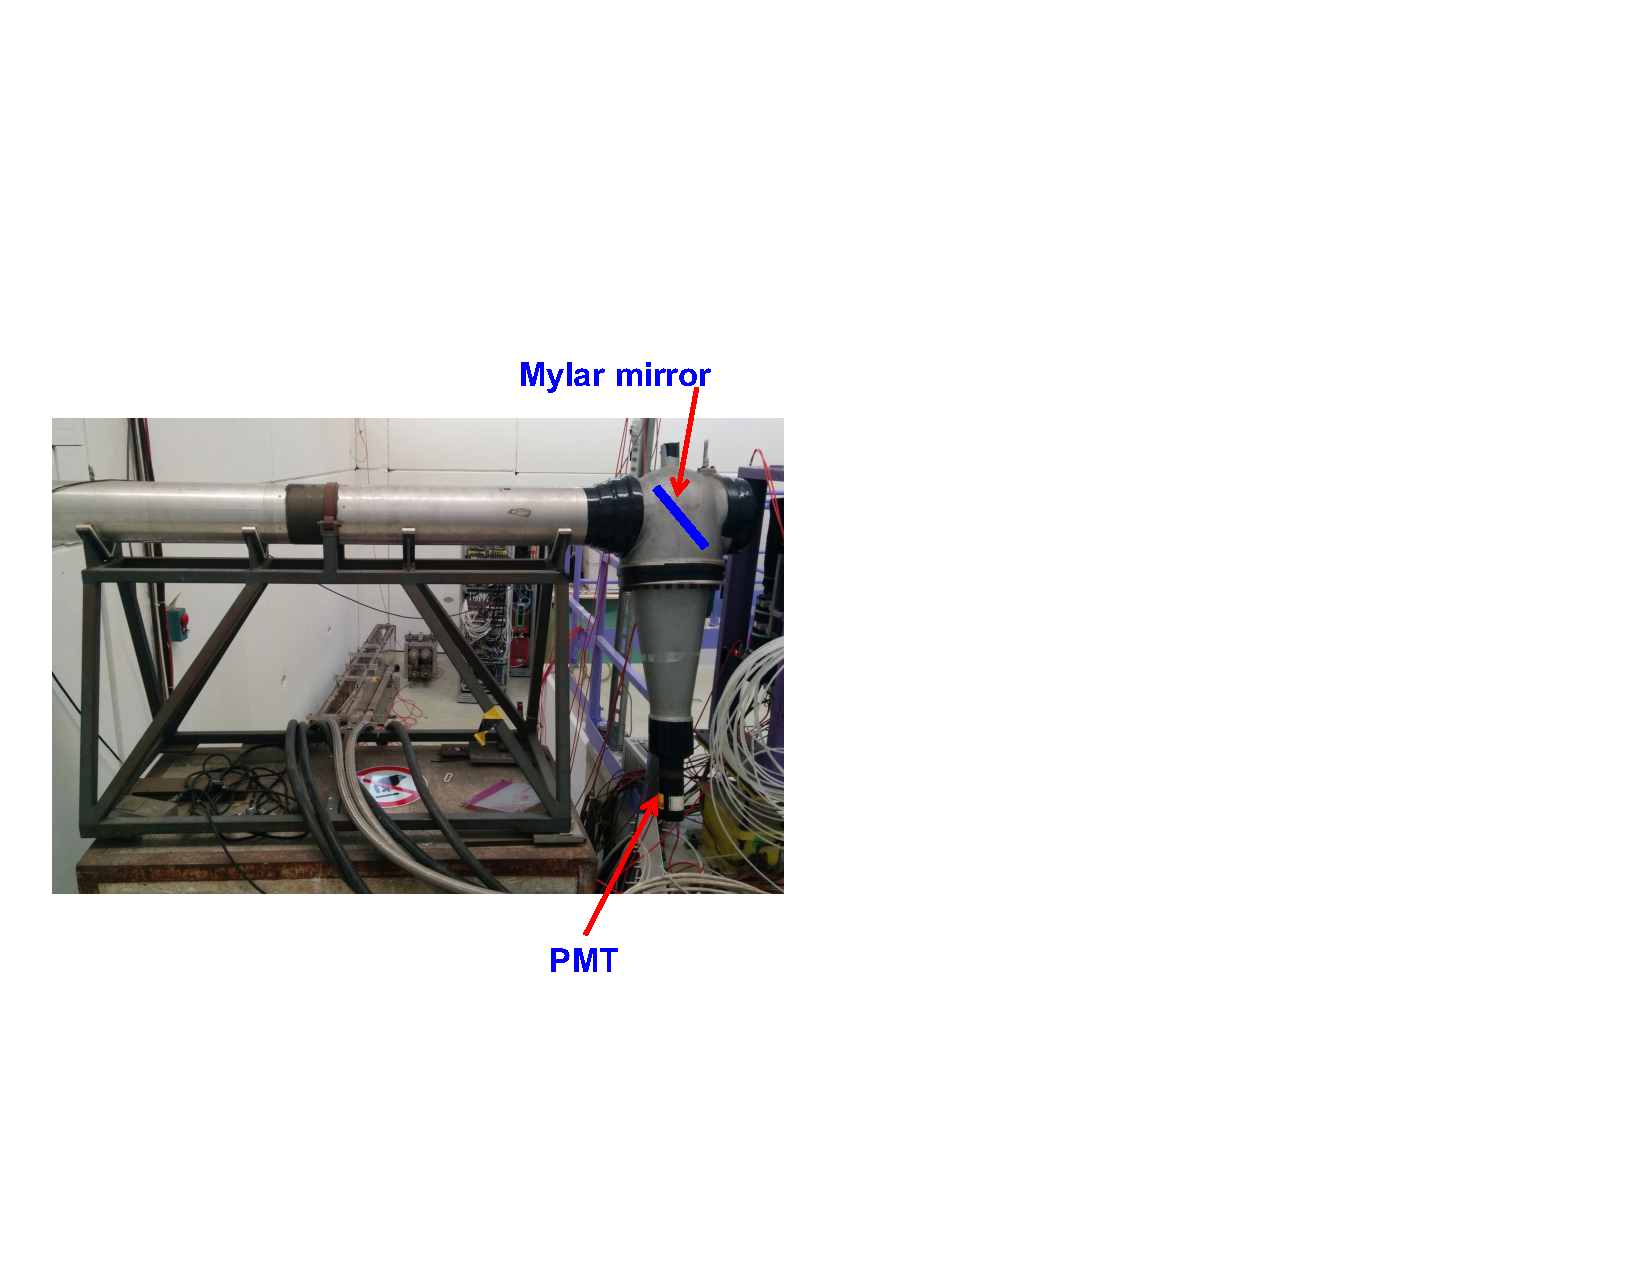
\includegraphics[width=0.65\textwidth]{beamline_ckv.pdf}
\end{cdrfigure}
\begin{cdrfigure}[Cherenkov gases]{ckv_gases}{Gas pressure threshold for the production of Cherenkov light for various particles as a function of particle momentum for Freon 12~\footnote{N. Charitonidis, Y. Karyotakis \it{et al.}, ``Hadron identification proposal for the ProtoDUNE experiments of CENF, to be published.} and CO$_2$ gases.}
  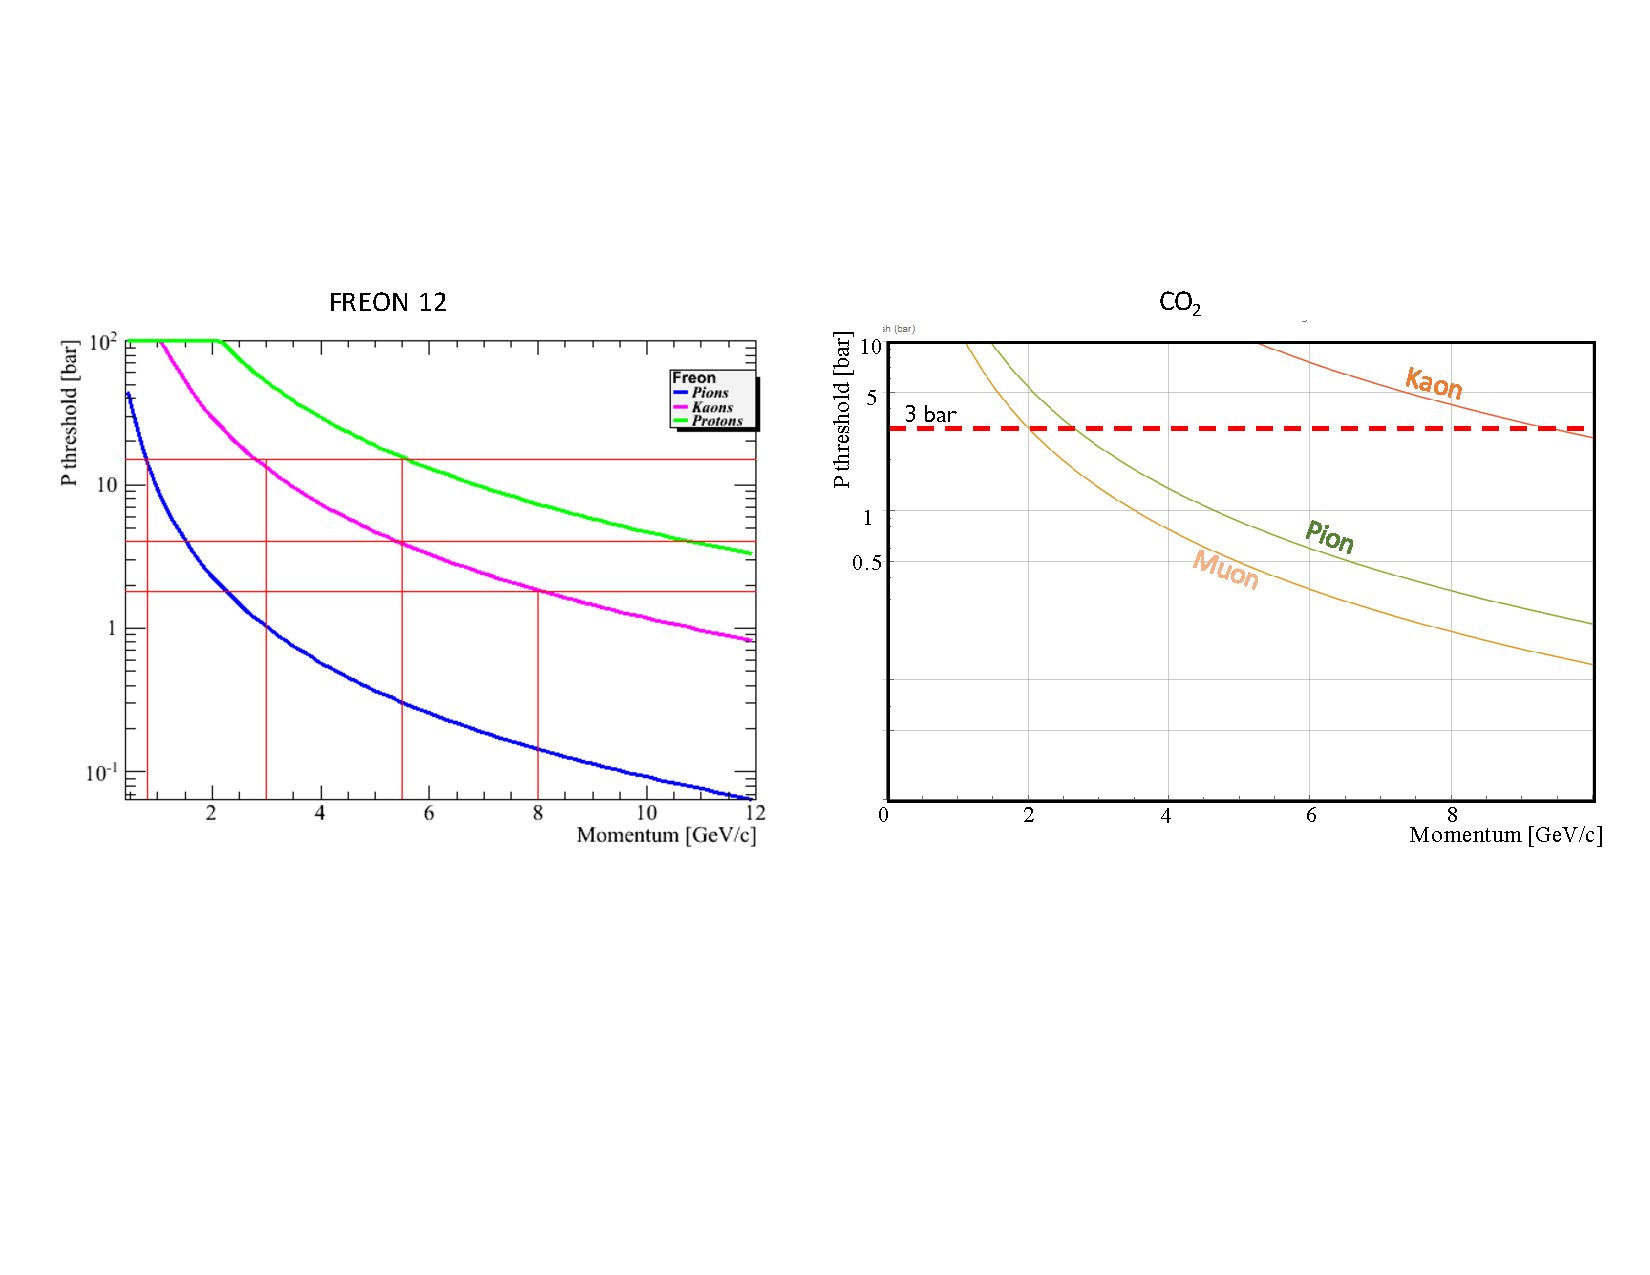
\includegraphics[width=0.99\textwidth]{beamline_CKVgases.pdf}
\end{cdrfigure}
Freon-12 has been selected for its high density, however it cannot be operated at pressures larger than 3bars to avoid liquefaction.  CO$_2$ can be used more easily at higher pressures.  

 Figure~\ref{fig:ckv_gases} shows that pions can be tagged with a 3bars Freon counter for momenta larger that 2 GeV/c, and Kaons can be tagged with an high pressure  (15~bars) CO$_2$  counter above 4 GeV/c.
%\fixme{Figure actually stops at 10 bar for CO2 ... either modify figure or text} 

The baseline plan for beam instrumentation includes a 2~m long
Cherenkov  counter filled with Freon-12 at adjustable pressure up to
3~bars (XCET1), and a  2~m long  
 Cherenkov  counter filled with CO$_2$ at adjustable pressure up to
 15~bars (XCET2).\\
%%
Existing Cerenkov counters at CERN are designed for pressures lower than  3~bar, therefore a new counter has to be manufactured in order to reach the 15 bars needed to efficiently tag Kaons. Drawings for such high pressure Cherenkov counters do exist since they were already used in the past. \\
%
Since both  counters will not be needed at all energies, the CO$_2$
counter, filled at low pressure,  will be used for electron discrimination at beam momenta lower
than 4GeV/c.  

A time-of-flight (ToF) system  is  necessary   to distinguish hadrons below the mentioned thresholds.
%
In summary:
\begin{itemize}
\item {\bf below 2~GeV/c} : one Cherenkov, filled with CO$_2$ low
  pressure, discriminates electrons. ToF needed for hadrons.
\item {\bf 2-3~GeV/c} : one Cherenkov, filled with CO$_2$ low
  pressure, discriminates electrons. Second Cerenkov, filled with
  Freon-12, tags pions. Kaons are negligible.
\item {\bf 3-4~GeV/c} : one Cherenkov, filled with CO$_2$ low
  pressure, discriminates electrons. Second  Cherenkov, filled with
  Freon-12, tags pions. ToF is needed for Kaon/proton discrimination
\item {\bf 4-7~GeV/c} : one Cherenkov, filled with CO$_2$ high
  pressure, tags Kaons. Second  Cherenkov, filled with
  Freon-12, tags pions. Electron content of the beam is low and can be
  discriminated by reconstruction.
\end{itemize}


%\fixme{Above paragraph needs to be rewritten more clearly. As written it is confusing.}

  From table \ref{tab:beampartcomp} it is evident that the Kaon content of the beam is negligible at least below 2 GeV/c, thus  only pion-proton separation is needed at low energies. Figure\ref{fig:toftau} shows the ToF resolution needed to distinguish among particle species at the $4\sigma$ level as a function of the particle momentum, assuming a 23~m long path. To distinguish pions from protons below 2 GeV/c a 1~ns resolution is enough, while 300ps are necessary for kaon-proton up to  4~GeV/c. It has also to be noted that a ToF system with a ~100ps resolution would allow to identify protons from other hadrons up to 7~GeV, so that the high pressure CO$_2$ Cherenkov could be avoided. Conversely, in order to cover all the energy range up to 7~GeV for all hadron  types, a ToF system with a resolution better than 40~ps would be needed.
In the following, two (possibly complementary) ToF systems are described.
\begin{cdrfigure}[Required ToF resolution]{toftau}{Required ToF resolution to  distinguish among particle species at the $4\sigma$ level as a function of the particle momentum, assuming a 23~m long path. }
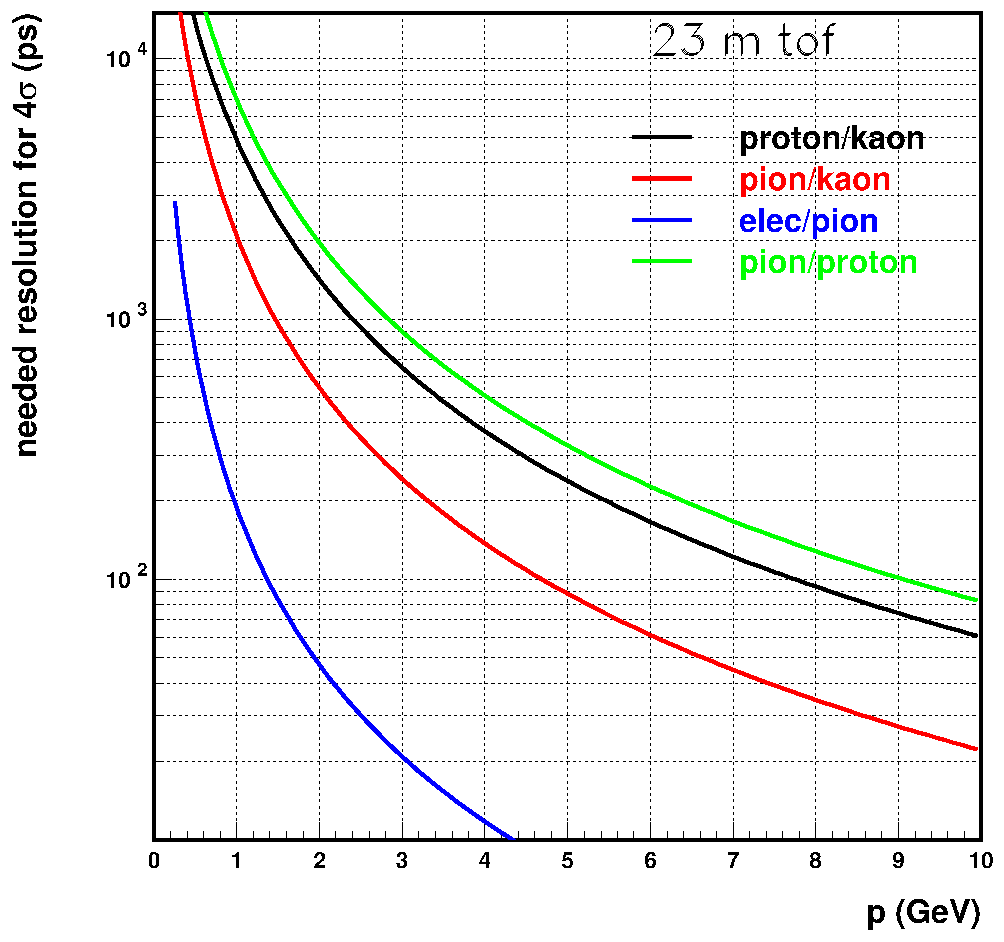
\includegraphics[width=0.65\textwidth]{toftaulow.pdf}
\end{cdrfigure}
%\fixme{Enlarge axis labels and tick marks so that figure can be reduced in size and still be legible.}

\paragraph{pLAPPD Time-of-flight system}
FermiLab is testing a ToF system that would utilize a 6 x 6 cm$^2$
large-area picosecond photodetectors (pLAPPDs) as shown in figure \ref{fig:pLAPPD}.
 The MCP-based devices
are capable of $< 50$~ps resolution with gains of $10^6-10^7$,
mm-position resolution along one axis and slightly worse resolution
along the other axis.  The photodetector is mounted on a readout
board, so the relevant exterior dimensions are 165.1mm x 109.3mm and a
thickness of 16mm. The active area is defined by the 4 squares visible in figure \ref{fig:ppLAPPD}, and amounts to about 8~cm$^2$. Tests of these devices in the Lariat beam are underway, to precisely assess the timing capabilities.
\begin{cdrfigure}[pLAPPD]{pLAPPD}{Photo of one pLAPPD device as proposed for the H2 and H4 beamlines.}
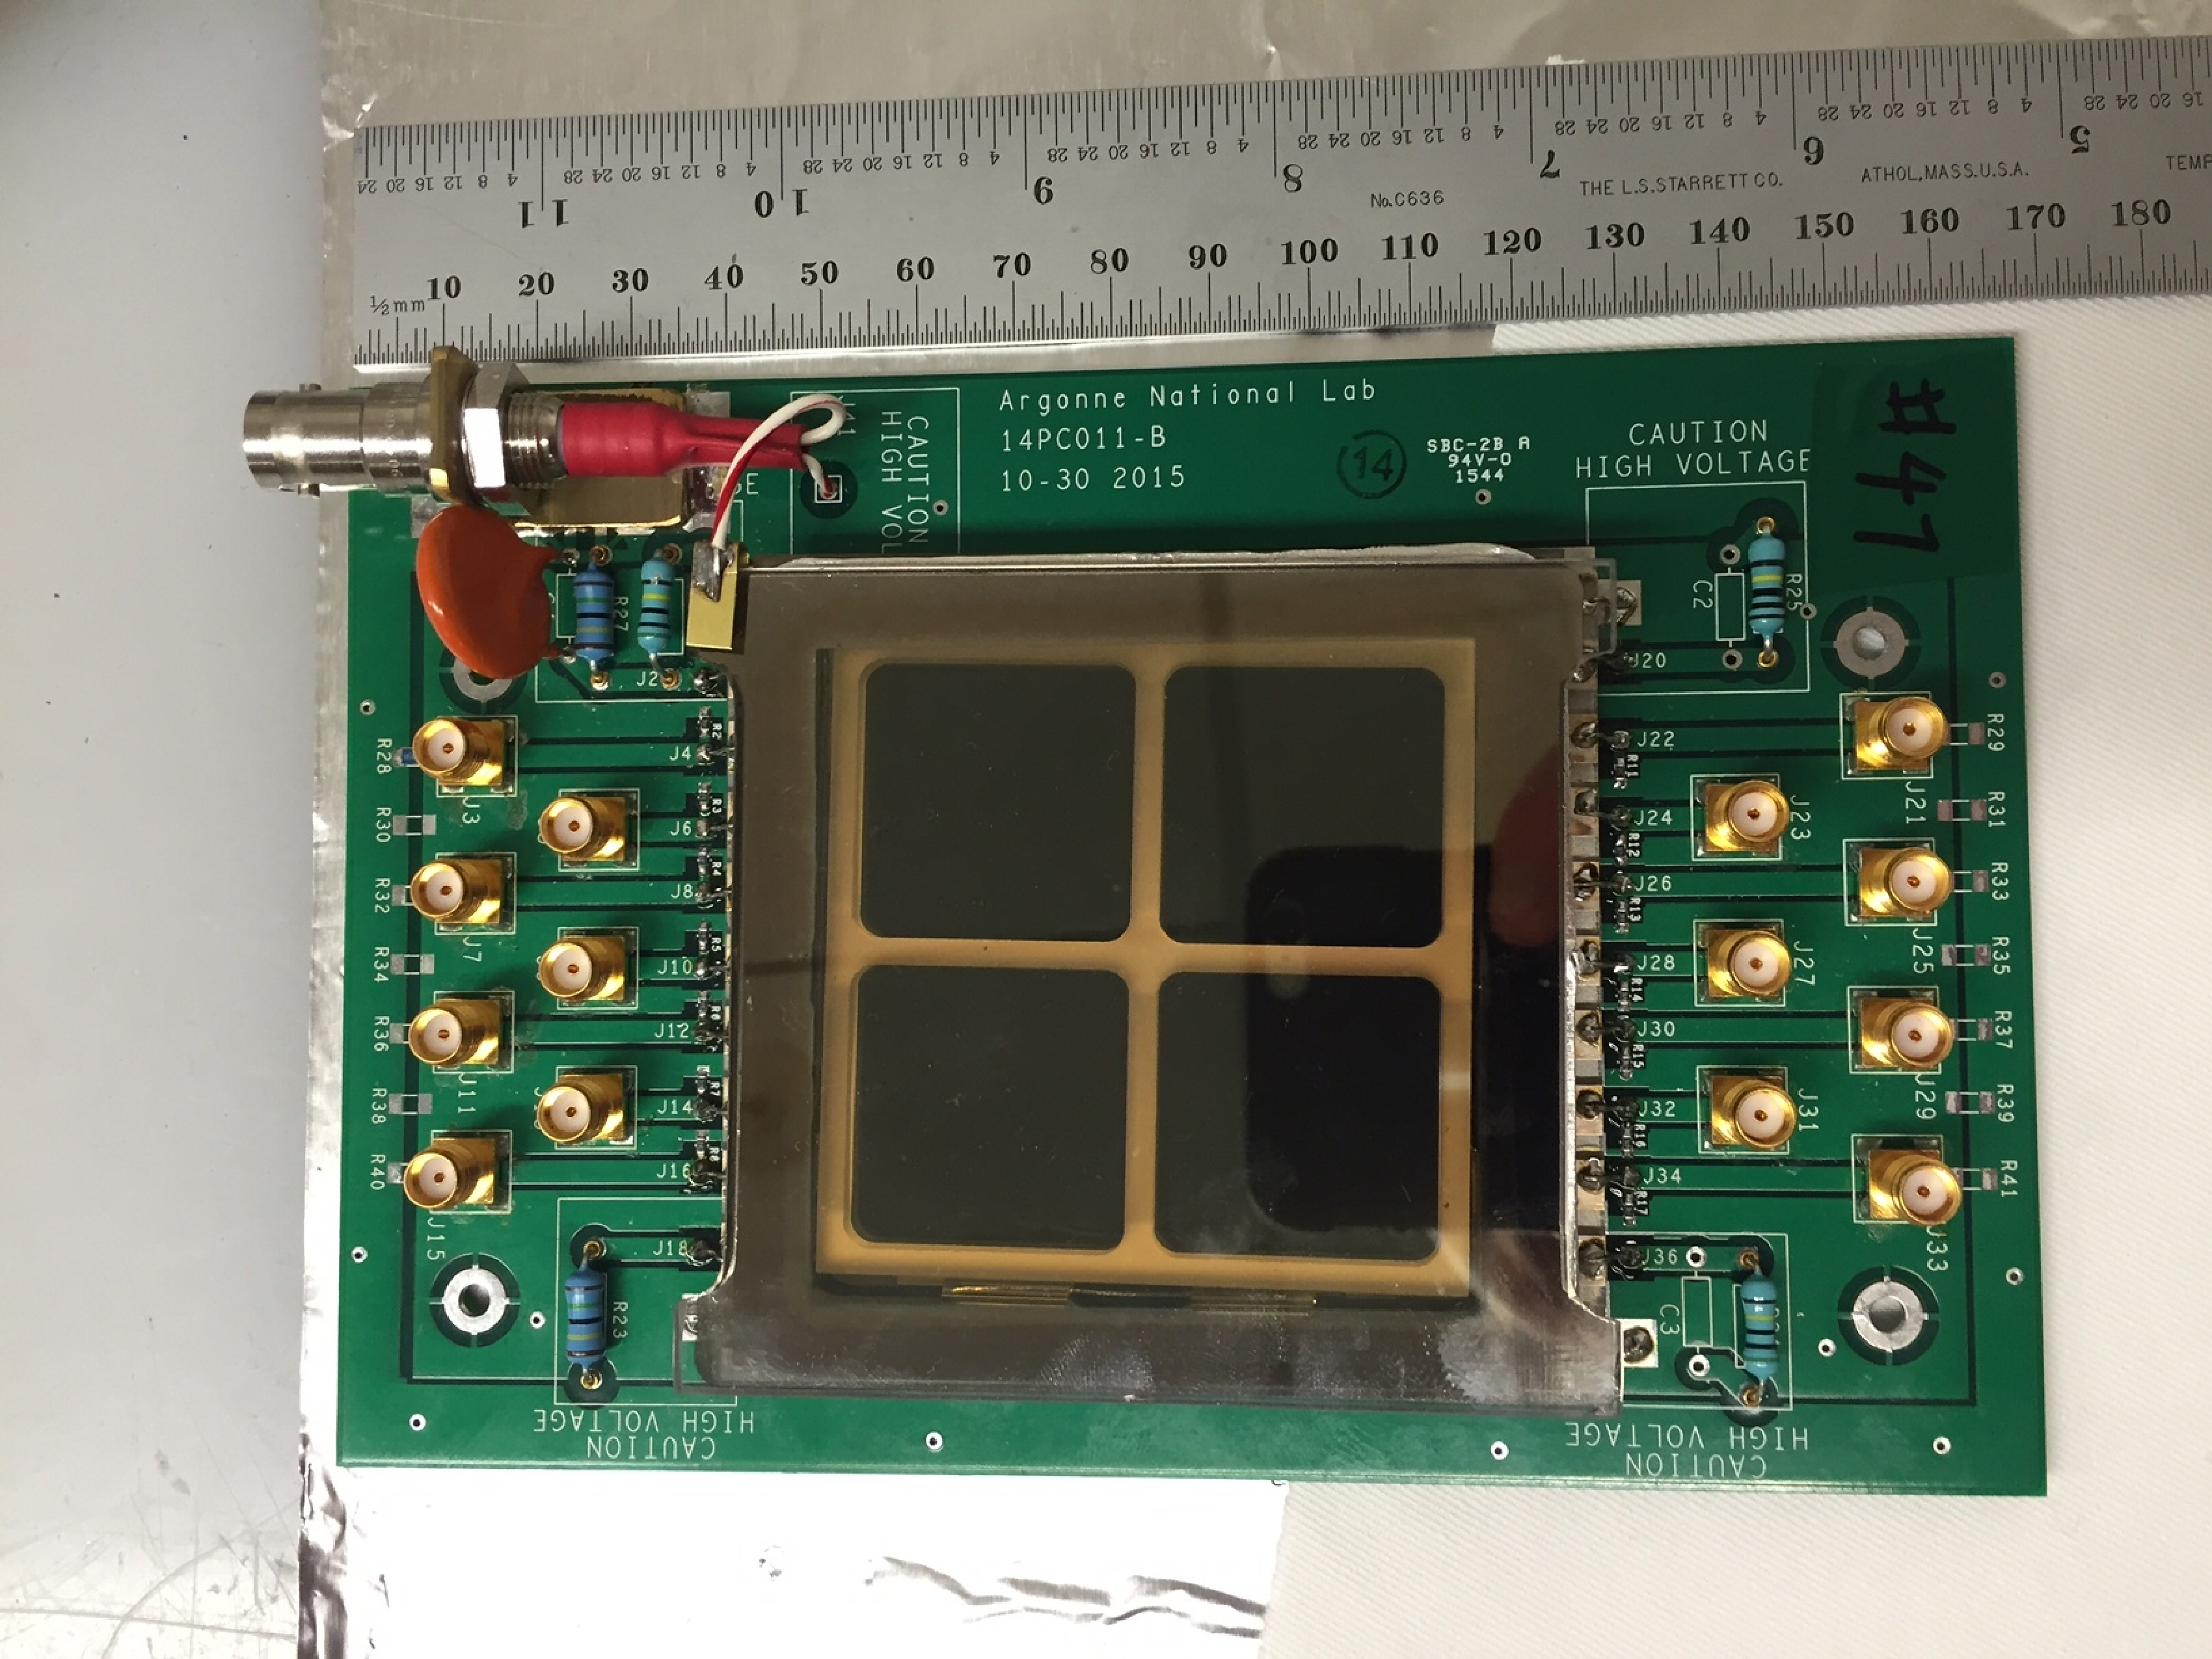
\includegraphics[width=0.65\textwidth]{LAPPD.pdf}
\end{cdrfigure}

\paragraph{Other Time-of-flight system}
The  scintillating fiber monitors can be used also for ToF purposes with the goal of a 1~ns timing resolution, suitable for low (2$<$GeV/c) energy beams. The idea is to readout the detectors with the STiC ASIC\ref{STIC} for SiPM readout.
%%%, developed at the  Kirchhoff Institute for Physics in Heidelberg - will be clear from reference
In this configuration, the time resolution would be dominated by the fiber response. MonteCarlo simulations foresee a resolution better than 1~ns. 
A small prototype will be built and tested in the next few months to fully validate this solution.

%\fixme{Overall the beamline instrumentation section could benefit from a more clearly stated plan. The reader is left to guess what will and will not be built.}
%%%% done above and below

%%%%%%%%%%%%%%%%%%%%%%%
\subsection{Material Budget and discussion}
\label{beam-material-budget}
The choice of the ToF system, and the actual configuration of the beamline at each point in momentum depend also on the material budget. As described in the following, some of the instrumentation will have to be removed, or at least emptied, when operating below $\approx$~2 GeV. Also, the ToF system will be different for the low energy range.

Summing up all the required instrumentation, the ``full'' beamline will  include
%\fixme{should include OR will include ?? see earlier comments about 2nd Cherenkov counter. TOF counters ...}
%\fixme{not all the instruments are there all the time. I was not clear, try to do better}
 5 beam monitors (2 for tracking and 3 for spectrometry), two ToF devices, two 2~m long Cherenkovs at high density or pressure. The material budget would be much too high for operation at low momenta (below 2 GeV/c), 
% \fixme{quantify what "low" means}
 and in general for operation with electron beams.  
A full FLUKA\cite{fluka05,Fluka15}  simulation of materials in the beamline and of the ProtoDUNE detector, including the beam window details, has been used to evaluate the effect of materials and are presented here. 
%\fixme{Should also mention that a second simulation was performed using GEANT 4 and that consistent results were obtained. }
%\fixme{ I saw no GEANT4 simulation with the beam instrumentation, except the one, very recent, from Nikos. And I would like to keep the ``materials etc'' simulations on the Protodune side, not on the Beam group. Conversely, I saw at the workshop strange GEANT4 results with a wrong geometry of the beam window. If you refer to the old work done last year, the materials have changed.}
Earlier material studies with Fluka have been compared with GEANT 4 based results and good agreement was found. More recent GEANT 4 based studies are still in progress.

Since the final layout of the beamline optics was delivered only recently, the simulations presented here assume a straight line with an initially parallel beam, deflected only by scattering. Particles are assumed to be ``lost'' when scattered outside of the beam pipe. Implementation of the magnetic elements is underway.
 Figure~\ref{fig:matblfull} shows the evolution of the material budget with a full instrumentation, assuming pLAPPD for ToF. The total, including the beam window, would add $0.6X_0$, 0.15 interaction lengths, and an energy loss for a mip of 28~MeV.
The largest energy loss contribution comes from Cherenkov detectors and from the  ToF system. Cherenkovs are not particularly useful for low energies (except a low-pressure one for electron discrimination), can be easily removed from the beamline and substituted with a section of vacuum pipe, or emptied.  
In a situation without Cherenkovs, the pLAPPD devices plus monitors would still account for almost  $0.2X_0$. Besides energy degradation, scattering of low energy particles would  further degrade the pion and proton content of the beam.  Figure~\ref{fig:1GeVtof} show examples of the beam degradation due to materials at 1~GeV/c: The rate of pions arriving at the detector is reduced by a factor 2.5, and the energy spread rises to 1.2\%. The rate of protons stopping in the detector is reduced by a factor 4, and the energy spread amounts to 2\% rms. This calculation is done in optimistic conditions, that is neglecting the efficiency loss due to the small active area of the pLAPPD devices.

To overcome this problem, it is foreseen to   use  scintillating fibers as ToF devices for the lowest energy beams ($< 2 GeV$), and pLAPPD above 2~GeV.
   This will require reconfiguration of the beamline, and needs to be carefully considered in the run plan, but it is feasible.  
%\fixme{Has this been decided ? What is the plan ??}
%%%\fixme{It is decided, pending tests with a prototype, purchase of electronics started}
 %The feasibility of a fully plug-and-play beamline, with detectors going in and out, including those that need vacuum segmentation, is under discussion. 
 %\fixme{In TDR cannot say that it is under discussion; need a baseline solution and possibly an alternate solution.}
 


It has also to be noted that a good performance of the (combined) ToF system could avoid the use of high pressure  Cherenkov counters. This option is not considered here, but could
represent an important simplification  in case the pLAPPD tests will demonstrate a resolution of $\approx$20ps.
%\fixme{What are "non-standard" Cherenkov counters ?? High pressure, Freon...}
 \begin{cdrfigure}[Material budget]{matblfull}{Material budget in the beamline, as a function of the distance from the center of the detector (in cm). The red line describes the amount of $X_0$, the black line the amount of interaction length, both read on the left axis. The black dotted line is the average energy lost by a mip particle, and is read on the right axis (in MeV). Vertical lines show the positions of the various beam monitors (in between the two blue lines are the 3 devices for spectrometry, ``bm'' is the last beam monitor, ``bw'' is the starting point of the beam window).}  
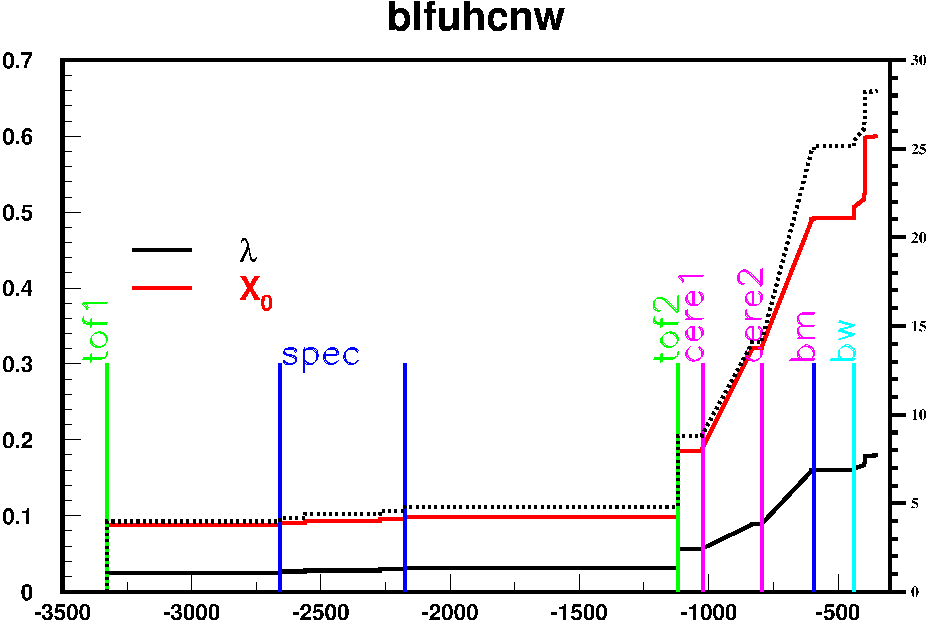
\includegraphics[width=0.65\textwidth]{blfuhcnwrayplo.pdf}
\end{cdrfigure}
%\fixme{remove funny title of plot; add axes labels}
%
 \begin{cdrfigure}[Effect of materials at  1GeV]{1GeVtof}{Effect of materials at  1GeV/c. Left: $\pi$ beam, energy of the particle entering in the detector, in three conditions: with  beam monitors, with beam monitors and pLAPPD for ToF, with the whole beamline filled with air (and no instrumentation). Right: proton beam, energy deposited by protons stopping in the LAr active volume, in three conditions: without instrumentation (the beam window is always present), with the scintillators only, and with scintillators plus pLAPPD for ToF.}
% \fixme{increase label size and possibly size of text in fig.} }
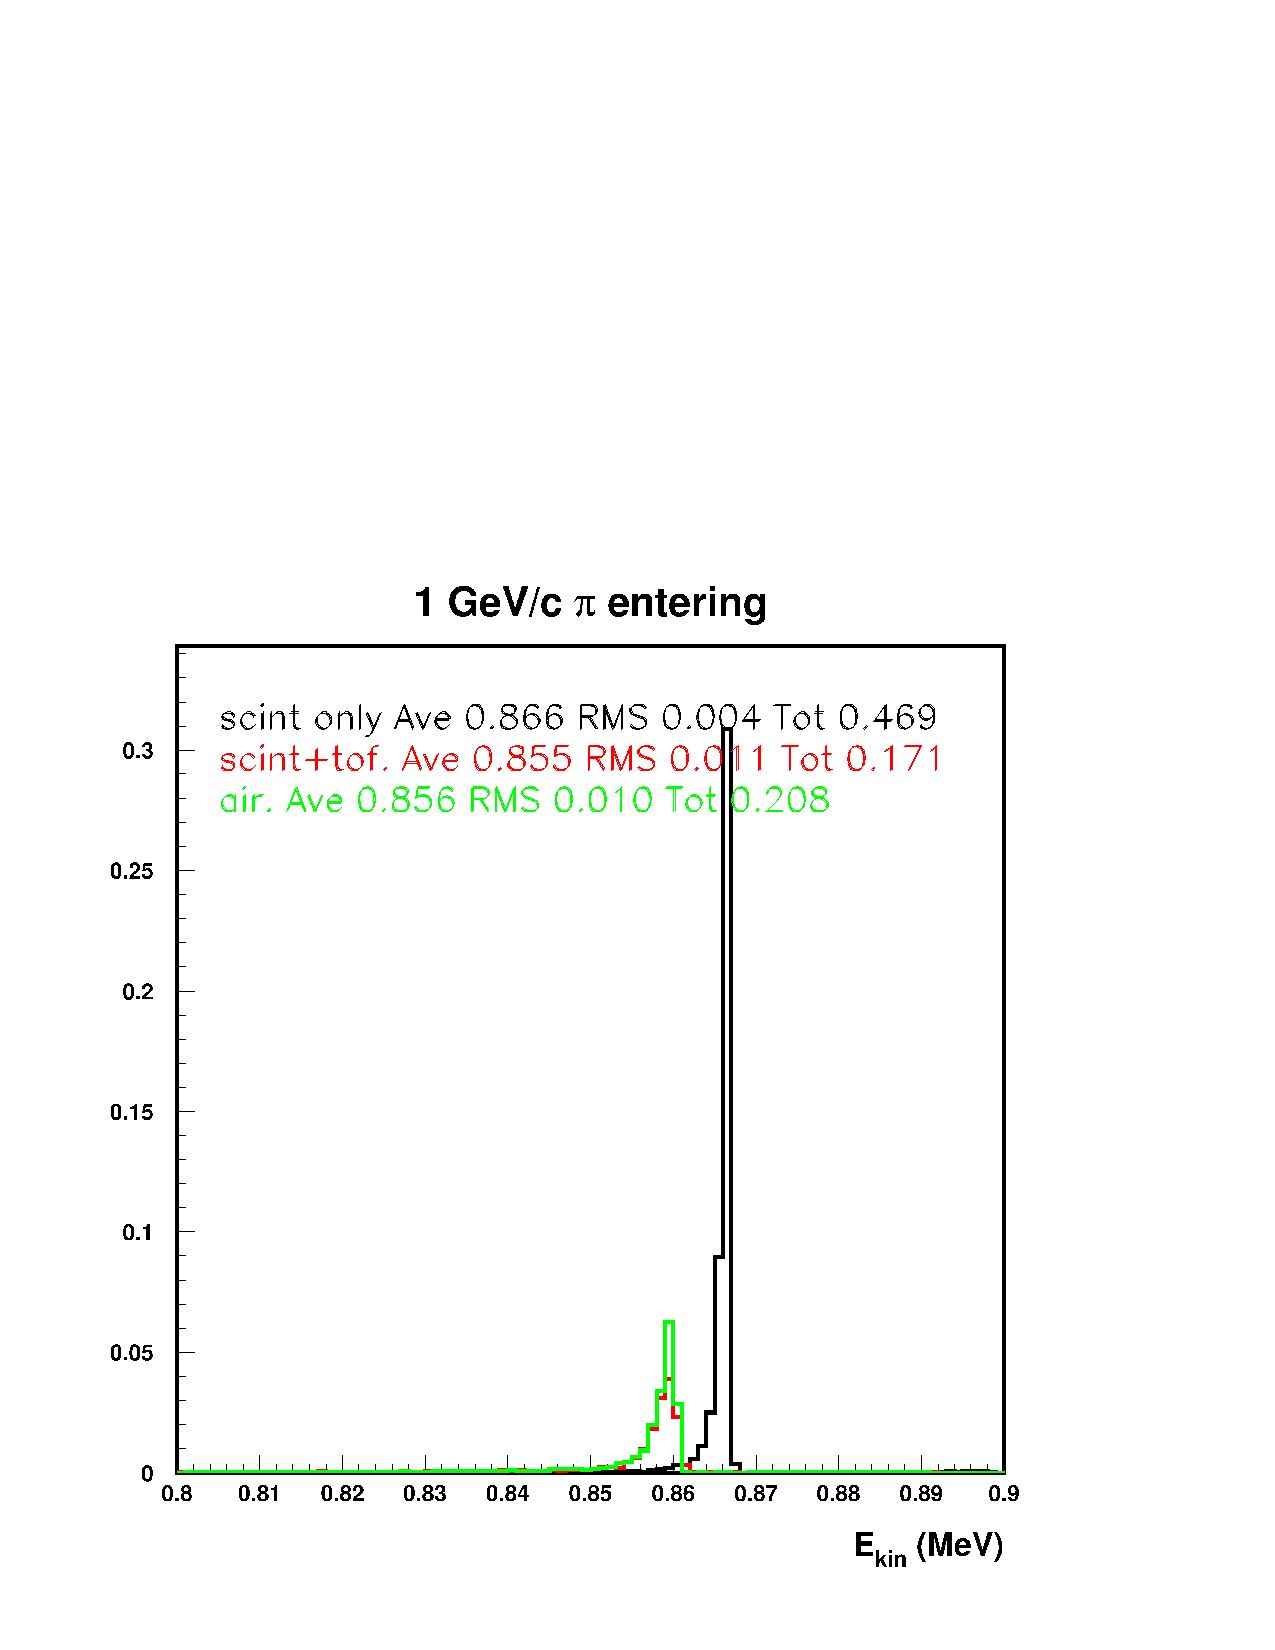
\includegraphics[width=0.45\textwidth]{pi1p0gev_innw.pdf}
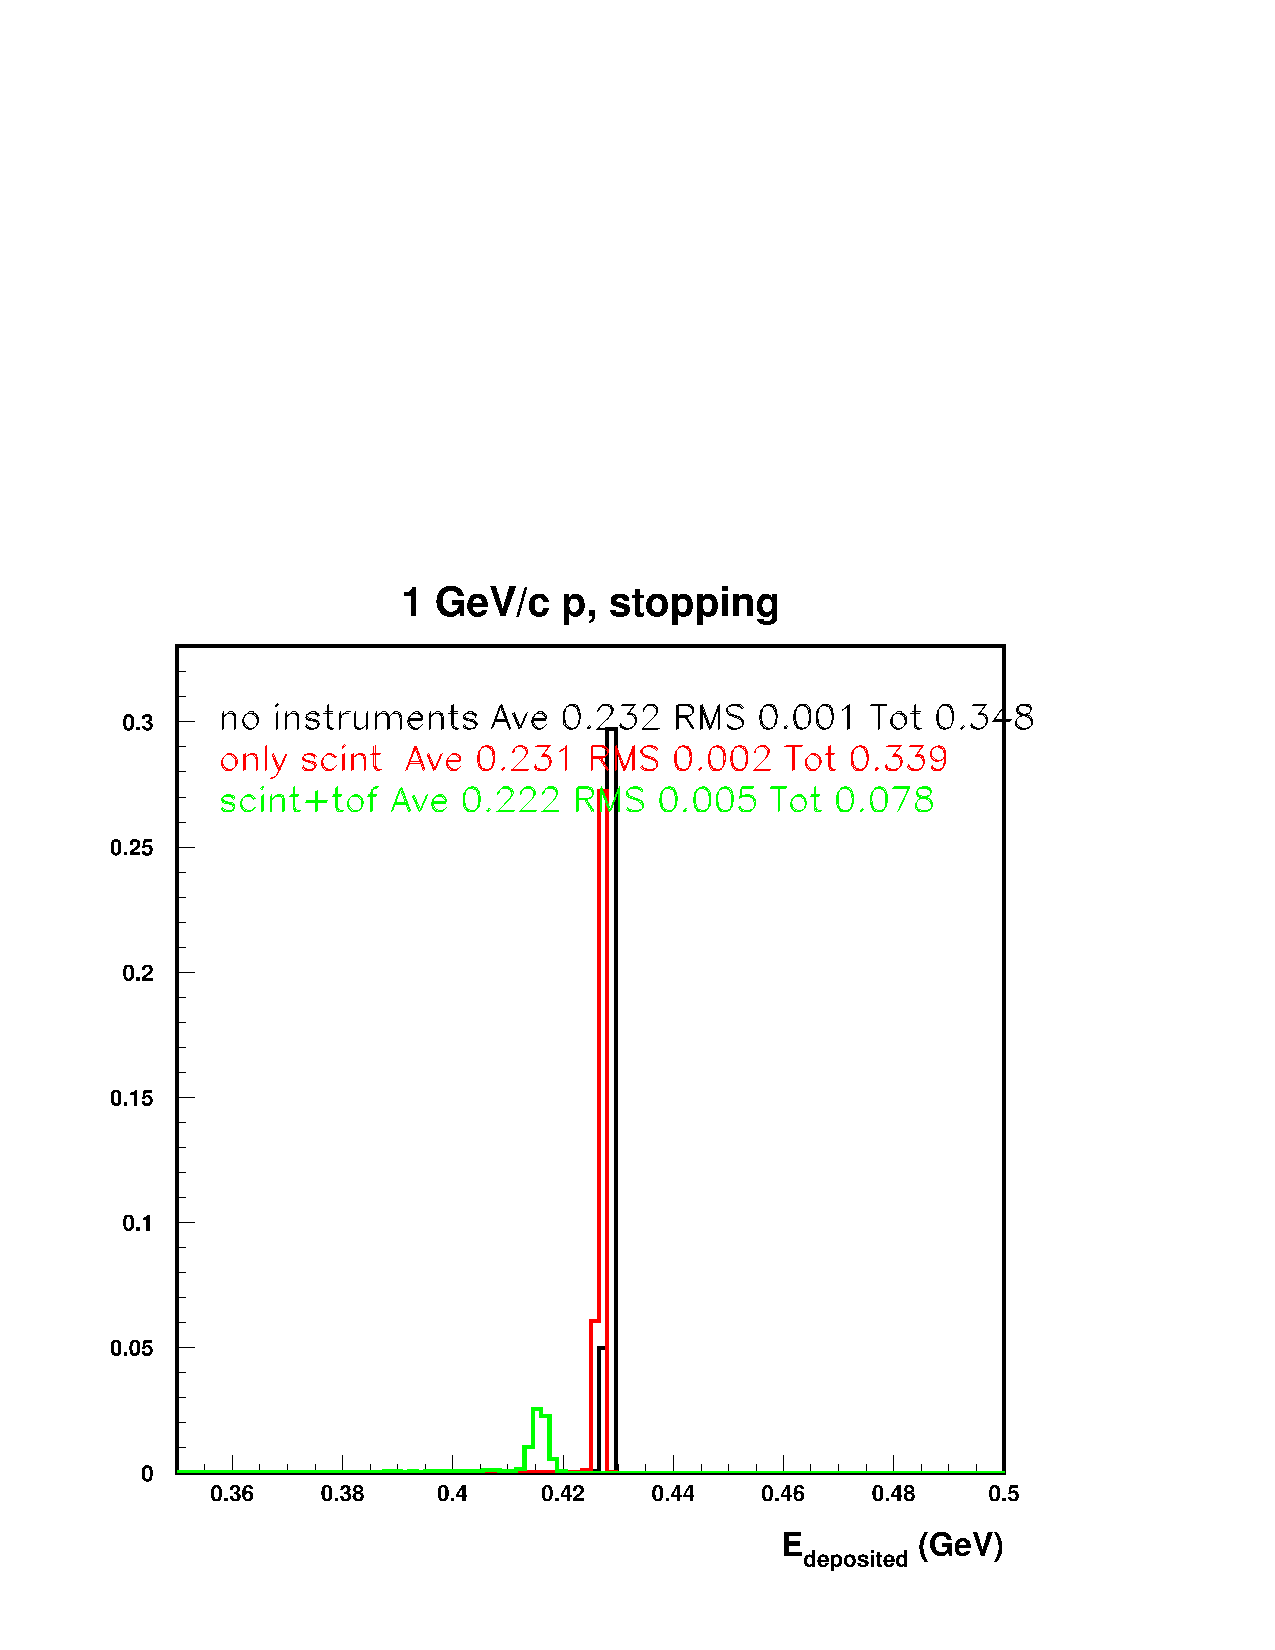
\includegraphics[width=0.45\textwidth]{p1gevstopnoqnw.pdf}
\end{cdrfigure}



%%%%%%%%%%%%%%%%%%%%%%%
\subsection {Trigger and data acquisition}
%Discussions are ongoing 
%%%\fixme{Once more: cannot say that discussions are ongoing ...}
%%\fixme{Thomas, you are right, but we got only last week a name for the responsibility of the trigger! And we had a more-or-less kickoff meeting last friday (AFTER writing this chapter), WITHOUT the responsible... }
The beam instrumentation will provide a trigger signal, built from the coincidence of the two last beam monitors, vetoed by the electron-tagging Cerenkov for low energy beams. A trigger mask, providing the status of the other counters, will also be provided. 
 Synchronization of the Detector DAQ with the beam instrumentation DAQ will be ensured by a common time stamp through a White Rabbit network.
%%%\fixme{Has white rabbit been agreed on ?}
%%%\fixme {YES}
 White Rabbit is a fully deterministic Ethernet-based network for general purpose data transfer and synchronization. It can synchronize over 1000 nodes with sub-ns accuracy over fiber lengths of up to 10 km. It is developed and widely used at CERN.

Beam instrumentation data will be readout independently on a separate DAQ stream. However,  
the beam data fragments corresponding to  events with a valid trigger from both beam and ProtoDUNE will be merged online with the detector data.
 
